\pagebreak
\subsection{Implementing V-Cycle Multigrid Method}

%\textcolor{red}{Implement a V-cycle multigrid method that will work starting from an arbitrary grid level p, with two or more grid levels. Describe your implementation, including the restriction and prolongation operators.}

    %\textcolor{red}{[7pts] Plot the $L_2$ residual norm convergence of the multigrid method (norm versus multigrid iteration) with a fixed coarse grid of $p = 1$, for 2, 3, 4, and 5 levels. How does the convergence rate behave as the number of levels is increased?}

The method of the V-Cycle multigrid is computing the residual at a fine mesh, restricting it to a smaller grid then repeating until reaching the coarsest mesh grid size. At this coarsest meshgrid the restricted residual will be smoothed and then the prolongation scheme will start. In this prolongation the error is passed up through each prolongation and smoother and ultimately added to the initial guess of the state matrix.

    \subsubsection{V-Cycle Multigrid Method Convergence}
    \paragraph{Restriction}
    Restricting the multigrid can be done by simply iterating by multiples of 2 throughout the $x$ and $y$ directions and taking a weighted average of the surrounding nodes such that the restriction can be written below in Equation \ref{eqn:restrict},

        \begin{equation}
            r_{i,j} = \frac{1}{4}\underbrace{r_{i,j}}_{\text{Center node}} + \frac{1}{8}\underbrace{\left(r_{i\pm 1,j} + r_{i,j\pm 1}\right)}_{\text{Up/Down nodes}} + \frac{1}{16}\underbrace{\left(r_{i\pm 1,j\pm 1} + r_{i\pm 1,j\mp 1} \right)}_{\text{Corner nodes}}
            \label{eqn:restrict}
        \end{equation}\myequations{Full-Weighting Residual Restriction}

    \paragraph{Prolongation}
    Prolongation is similar to restriction except that it is acting in the opposite direction. Instead of weighting adjacent nodes to a center node it applies one node to several. In my implementation I would iterate fully through the finer mesh but I would conduct integer division to use values from every other node and then weight them accordingly. The expression that I used for prolongation can be shown below in Equation \ref{eqn:prolongation}

        \begin{equation}
            \begin{bmatrix}
                e_{i-1_{h},j+1_{h}} & e_{i_{h},j+1_{h}} & e_{i+1_{h},j+1_{h}}\\
                e_{i-1_{h},j_{h}} & e_{i_{h},j_{h}} & e_{i+1_{h},j_{h}}\\
                e_{i-1_{h},j-1_{h}} & e_{i_{h},j-1_{h}} & e_{i+1_{h},j+1_{h}}
            \end{bmatrix} = \begin{bmatrix}
                \frac{1}{4}e_{i_{2h},j_{2h}} & \frac{1}{2}e_{i_{2h},j_{2h}} & \frac{1}{4}e_{i_{2h},j_{2h}}\\
                \frac{1}{2}e_{i_{2h},j_{2h}} & e_{i_{2h},j_{2h}} & \frac{1}{2}e_{i_{2h},j_{2h}}\\
                \frac{1}{4}e_{i_{2h},j_{2h}} & \frac{1}{2}e_{i_{2h},j_{2h}} & \frac{1}{4}e_{i_{2h},j_{2h}}
            \end{bmatrix}
            \label{eqn:prolongation}
        \end{equation}\myequations{State/Error Prolongation}

    
    \paragraph{Implementing Multigrid}
    Using Equations \ref{eqn:restrict}, \ref{eqn:prolongation} and implementing into the Python environment with Algorithm \ref{alg:v_cycle}, I ultimately arrive to find the convergence rates for the V-Cycle multigrid. Running several iterations with differing $p$ values I get that the $L_2$ residual norms with $\nu_1=\nu_2=2$ and $\nu_c=50$ are shown in Figure \ref{fig:vcyc_l2_err} on the following page.

    \pagebreak
    \begin{figure}[h]
        \centering
        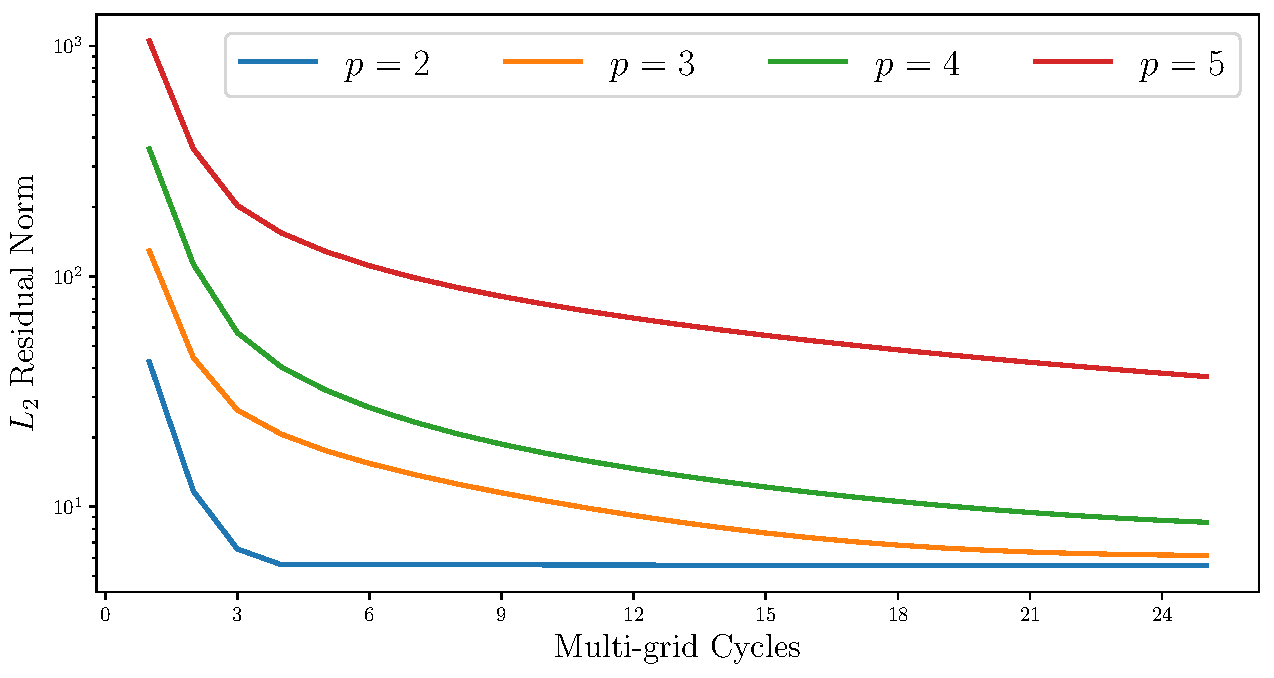
\includegraphics[width = 0.9\linewidth]{tasks/figs/vcyc_l2_err.pdf}
        \caption[V-Cycle $L_2$ Convergence]{The V-Cycle multigrid method $L_2$ convergence while varying $p$.}
        \label{fig:vcyc_l2_err}
    \end{figure}

    Shown above in Figure \ref{fig:vcyc_l2_err}, is the convergence for the V-cycle multigrid $L_2$ residual norm. Looking to the convergence rates, as you increase the size of the meshgrid (increase of $p$) the longer it will take to converge to the solution. This can be shown as the horizontal asymptote reached first from $p=2$. Noting that the $L_2$ residual norm is relatively large this is most likely due to the fact that the smoothing values $\nu_1, \nu_2,\nu_c$ are all relatively small compared to the actual smoothing iterations that I used for Jacobi and Gauss-Seidel with $\mathcal{O}(2500)$ iterations. These small smoothing values result in a larger residual but a converged solution nonetheless.



    \pagebreak
    \subsubsection{V-Cycle Multigrid Smoothing Iterations}
    %\textcolor{red}{[8pts] For $p = 0$ as the coarsest level and $p = 4$ as the finest, investigate the behavior of multigrid by varying pre/post/coarse smoothing iterations. Try to determine the most efficient setting of smoothing iteration numbers for multigrid, and make one or more plots with several convergence histories to demonstrate your investigation. For a fair comparison, plot the $L_2$ residual norm convergence against \textit{work units} (WU), where 1 WU corresponds to the cost of one smoothing iteration on the finest grid. Note that in this two-dimensional problem, going down to a coarser level decreases the cost of smoothing by a factor of 4. Also include (overlay) a convergence plot of pure GaussSeidel ($\omega = 1.5$) on the finest level for comparison.}

    In order to choose an efficient V-cycle setting to create accurate solutions that require lower computing power relative to other solutions will require ``\textit{tweaking}'' of the smoothing iterations until values are found that result in accurate solutions that require less computing than other alternatives. To relate V-Cycle multigrid to Gauss-Seidel I will be using Work Units to compare the two. The units for ``work units'' can be defined below in Equation \ref{eqn:workunits},

        \begin{equation}
            1\ \text{V Cycle} = \sum_{l=0}^{n_\text{level}-1}\left(\nu_1 + \nu_2\right)2^{-l}\  \text{Work Units}
            \label{eqn:workunits}
        \end{equation}

    After some trial and error and adjusting $\nu_1, \nu_2, \nu_c, $ and the number of iterations plotting V-Cycle multigrid and Gauss-Seidel against their work units arrives to Figure \ref{fig:vcyc_gs} shown below.

    \begin{figure}[h]
        \centering
        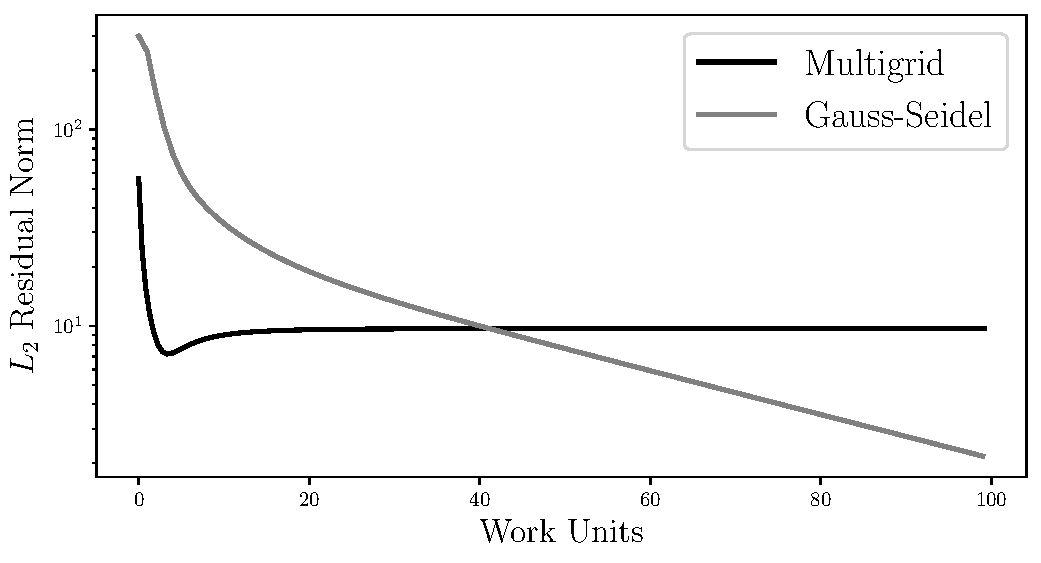
\includegraphics[width = 0.9\linewidth]{tasks/figs/vcyc_gs.pdf}
        \caption[V-Cycle Multigrid Smoothing Iterations]{Adjusting V-Cycle multigrid parameters to compare computational costs between V-Cycle multigrid and Gauss-Seidel smoother.}
        \label{fig:vcyc_gs}
    \end{figure}

    Looking above to Figure \ref{fig:vcyc_gs}, I found that the V-cycle was ultimately more accurate for lower work units but at higher work units Gauss-Seidel would become more accurate as V-cycle would start to bring diminishing returns at higher work units. I believe that this is due to the fact that this V-cycle multigrid would converge quickly to its solvers solution whereas the Gauss-Seidel methods solution is more accurate but for better accuracy costs significant more computational power(multigrid converged to its solution at $\approx$ 10 work units whereas it took Gauss-Seidel $\approx$ 40 work units). For quick convergence these are the V-Cycle multigrid smoothing parameters that I recommend.

    \begin{equation*}
        \boxed{\bf k = 50,\quad \nu_1 = 10,\quad \nu_2 = 10,\quad \nu_c = 1000}
    \end{equation*}